
\subsection{Soluci\'{o}n de sistemas tridiagonales}
\begin{frame}
\frametitle{Soluci\'{o}n de sistemas tridiagonales}
Una ecuaci\'{o}n tridiagonal la podemos escribir de la siguiente forma:
\[
\begin{bmatrix}
B_{1} & C_{1} & 0 & 0 & 0 & 0 \\
A_{2} & B_{2} & C_{2} & 0 & 0 & 0 \\
0 & A_{3} & B_{3} & C_{3} & 0 & 0 \\
0 & 0 & 0 & \ddots & 0 & 0 \\
0 & 0 & 0 & 0 & A_{n}& B_{n} 
\end{bmatrix}
\begin{bmatrix}
\phi_{1} \\
\phi_{2} \\
\phi_{3} \\
\ddots \\
\phi_{N} \\
\end{bmatrix} =
\begin{bmatrix}
D_{1} \\
D_{2} \\
D_{3} \\
\ddots \\
D_{N} \\
\end{bmatrix}
\]
\end{frame}
\begin{frame}
El algoritmo de soluci\'{o}n para esta matriz es el siguiente:
\begin{enumerate}
\item Se inicializan dos nuevas variables: $B'_{1}=B_{1}$ y $D'_{1}=D_{1}$.
\item Se calculan de forma recursiva las siguientes ecuaciones, de $i$ hasta $N$:
\[ \begin{split} R &= \dfrac{A_{i}}{B'_{i-1}} \\
B'_{i} &= B_{i} -RC_{i-1} \\
D'_{i} &= D_{i} - RD'_{i-1}, \hspace{1cm} i=2,3,\ldots,N
\end{split} \]
\end{enumerate}
\end{frame}
\begin{frame}
\begin{enumerate}
\setcounter{enumi}{2}
\item Se calcula la soluci\'{o}n para la \'{u}ltima inc\'{o}gnita
\[ \phi_{i} = \dfrac{(D'_{i}-C_{i}\phi_{i+1})}{B'_{i}}, \hspace{1.5 cm} i=N-1, N-2,\ldots,1\]
\end{enumerate}
\end{frame}
\begin{frame}
\frametitle{Ejercicio}
Determinar las ecuaciones en diferencias y su soluci\'{o}n para el siguiente problema con valores en la frontera:
\[ -2y''(x) + y(x) = e^{-0.2x} \]
con las condiciones de frontera
\[ \begin{split} 
y(0) &= 1 \\
y'(10) &= -y(10)
\end{split} \]
Supongamos que los intervalos de la ret\'{i}cula tienen longitud unitaria.
\end{frame}
\begin{frame}
\frametitle{Soluci\'{o}n}
En la siguiente figura se muestra la ret\'{i}cula
\begin{center}
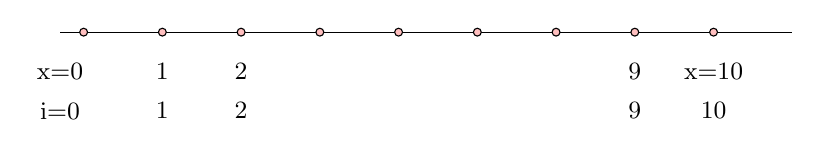
\begin{tikzpicture}[font=\small]
\draw (-1.3,0) -- (8,0);
\foreach \x in {-1,...,7}
	\draw [fill=red!25](\x,0) circle (0.05);
\draw (-1.3,-0.5) node {x=0};
\draw (0,-0.5) node {1};
\draw (1,-0.5) node {2};
\draw (6,-0.5) node {9};
\draw (7,-0.5) node {x=10};
\draw (-1.3,-1) node {i=0};
\draw (0,-1) node {1};
\draw (1,-1) node {2};
\draw (6,-1) node {9};
\draw (7,-1) node {10};
\end{tikzpicture}
\end{center}
Las ecuaciones en diferencias para $i=1$ hasta $i=9$, son:
\[ 2(-y_{i-1}+2y_{i}-y_{i+1}) + y_{i} = e^{-0.2i}, \hspace{1cm} x_{i}=i \]
\end{frame}
\begin{frame}
Para $i=1$, sustituimos la condici\'{o}n de frontera $y_{0}=y(0)=1$ en las ecuaciones anteriores, y resulta que:
\[ 5y_{1}-2y_{2} = e^{-0.2} +2\]
Para $i=10$, aproximamos la ecuaci\'{o}n diferencial por:
\[ - \dfrac{2(y'(10)- y'(9.5))}{\frac{1}{2}} + y(10) = e^{-2}\]
\end{frame}
\begin{frame}
Por medio de la aproximaci\'{o}n por diferencias centrales, el t\'{e}rmino $y'(9.5)$ es
\[ y'(9.5) = \dfrac{y(10)-y(9)}{1}\]
Sustituimos el resultado anterior y la condici\'{o}n de frontera $y'(10)=-y(10)$, para obtener
\[ -2y_{9} + 4.5y_{10} =  0.5 e^{-2} \]
\end{frame}
\begin{frame}
Las ecuaciones en diferencias son entonces
\[ \begin{split}
5y_{1} - 2y_{2} &= e^{-0.2} +2 \\
-2y_{i-1} + 5y_{i} - 2y_{i+1} &= e^-0.2x_{i}, \hspace{1cm} i=2,\ldots,9 \\
-2y_{9} + 4.5 y_{10} &= 0.5 e^{-2}
\end{split} \]
Donde $x_{i}=i$
\end{frame}
\begin{frame}
La matriz tridiagonal es
\[ \tiny{\begin{bmatrix}
5 & -2 & 0 & 0 & 0 & 0 & 0 & 0 & 0 & 0 \\
-2 & 5 & -2 & 0 & 0 & 0 & 0 & 0 & 0 & 0 \\
0 & -2 & 5 & -2 & 0 & 0 & 0 & 0 & 0 & 0 \\
0 & 0 & -2 & 5 & -2 & 0 & 0 & 0 & 0 & 0 \\
0 & 0 & 0 & -2 & 5 & -2 & 0 & 0 & 0 & 0 \\
0 & 0 & 0 & 0& -2 & 5 & -2 & 0 & 0 & 0 \\
0 & 0 & 0 & 0 & 0 & -2 & 5 & -2 & 0 & 0 \\
0 & 0 & 0 & 0 & 0 & 0 & -2 & 5 & -2 & 0 \\
0 & 0 & 0 & 0 & 0 & 0 & 0 & -2 & 5 & -2 \\
0 & 0 & 0 & 0 & 0 & 0 & 0 & 0 & -2 & 4.5 
\end{bmatrix}
\begin{bmatrix}
y_{1} \\
y_{2} \\
y_{3} \\
y_{4} \\
y_{5} \\
y_{6} \\
y_{7} \\
y_{8} \\
y_{9} \\
y_{10} \\
\end{bmatrix} =
\begin{bmatrix}
e^{-0.2}+2 \\
e^{-0.2x_{2}} \\
e^{-0.2x_{3}} \\
e^{-0.2x_{4}} \\
e^{-0.2x_{5}} \\
e^{-0.2x_{6}} \\
e^{-0.2x_{7}} \\
e^{-0.2x_{8}} \\
e^{-0.2x_{9}} \\
0.5e^{-2}
\end{bmatrix}} \]
\end{frame}
\begin{frame}
\frametitle{Soluci\'{o}n}
Implementando el c\'{o}digo en Python, tenemos los siguientes valores
\\
\medskip
\begin{minipage}{4cm}
\begin{tabular}{c | c}
ret\'{i}cula & soluci\'{o}n \\ \hline
0 & 1.00000000 \\
1 & 0.84643489 \\
2 & 0.70672186 \\
3 & 0.58520973 \\
4 & 0.48189665 \\
5 & 0.39486742 \\
\end{tabular}
\end{minipage}
\hspace{0.5cm}
\begin{minipage}{4cm}
\begin{tabular}{c | c}
ret\'{i}cula & soluci\'{o}n \\ \hline
6 & 0.32133217 \\
7 & 0.25786591 \\
8 & 0.20003411 \\
9 & 0.14127111 \\
10 & 0.07049423 \\
 & 
\end{tabular}
\end{minipage}
\end{frame}